\documentclass[a4paper]{article}

%\usepackage[utf8]{inputenc}

\usepackage{hyperref}
\usepackage{xcolor}
\usepackage{graphicx}
\usepackage[english]{babel}
\usepackage[T1]{fontenc}
\usepackage{url}
\usepackage{import}
\usepackage{multirow}
\usepackage{color}
\usepackage{fancyhdr}
\usepackage{amssymb}

\usepackage{mathtools}
\usepackage[margin=2.5cm]{geometry}
\usepackage{listings}
\usepackage[utf8x]{inputenc}
\usepackage[numbered,framed]{matlab-prettifier}

\let\ph\mlplaceholder % shorter macro
\lstMakeShortInline"

\lstset{
  style              = Matlab-editor,
  basicstyle         = \mlttfamily,
  escapechar         = ",
  mlshowsectionrules = true,
}


\begin{document}


\title{Elaborato di \\ \textbf{Calcolo Numerico}}

\author{Giovanni \emph{Bindi} - \texttt{5530804} - \href{mailto:giovanni.bindi@stud.unifi.it}{\textit{giovanni.bindi@stud.unifi.it}}
   \and Gabriele \emph{Gemmi} - \texttt{5602433} -
   \href{mailto:gabriele.gemmi@stud.unifi.it}{\textit{gabriele.gemmi@stud.unifi.it}}
   \and Gabriele \emph{Puliti} - \texttt{5300140} - \href{mailto:gabriele.puliti@stud.unifi.it}{\textit{gabriele.puliti@stud.unifi.it}}}

\maketitle

\tableofcontents


\newpage
\section{\textbf{Capitolo 1}}
\subsection{\textbf{Esercizio 1.1}}
Sapendo che il metodo iterativo è convergente a \( x^* \) allora per definizione si ha:
 \[
	\lim_{k \to +\infty}\ x_k = x^*
\]
 inoltre per definizione di \( \Phi \) si calcola il limite:
\[
    \lim_{k \to +\infty} \Phi(x_k) = \lim_{k \to +\infty} x_{k+1} = x^*
\]
 infine ipotizzando che la funzione \( \Phi \) sia uniformemente continua, è possibile calcolare il limite:
\[
    \lim_{k \to +\infty} \Phi(x_k) = \Phi(\lim_{k \to +\infty} x_k) = \Phi(x^*)
\]
 dai due limiti si ha la tesi:
\[
    \Phi(x^*) = x^* 
\]
\subsection{\textbf{Esercizio 1.2}}
Dal momento che le variabili intere di 2 byte in Fortran vengono gestite in Modulo e Segno, la variabile \texttt{numero} inizializzata con:
\begin{verbatim}
integer*2 numero
\end{verbatim}
varia tra \( -32768 \leq \texttt{numero} \leq 32767 \) (\( - 2^{15} \leq \texttt{numero} \leq 2^{15} - 1 \)). \\ 
Durante la terza iterazione del primo ciclo for si arriva al valore massimo rappresentabile tramite gli interi a 2 byte; alla quarta iterazione si avrà quindi la somma del \texttt{numero} in modulo e segno:
\[
(32767)_{10}+(1)_{10} = (0111111111111111)_{2,MS} + (0000000000000001)_{2,MS} = 
\] \( 
= (1000000000000000)_{2,MS} = (-32768)_{10} 
\) \\ \\
Nel secondo ciclo for, durante la quinta iterazione, al \texttt{numero} viene sottratto 1:
\[
(-32768)_{10}-(1)_{10} = (1000000000000000)_{2,MS} - (0000000000000001)_{2,MS} = 
\] \( 
= (0111111111111111)_{2,MS} = (32767)_{10} 
\) \\ \\
Da cui si spiega l'output del codice.
\subsection{\textbf{Esercizio 1.3}}
Per definizione si ha che la precisione di macchina \(u\), per arrotondamento e' data da:
\[
u=\frac{1}{2} b ^{1-m}
\]
Se \(b=8, m=5\) si ha:
\[ 
u = \frac{1}{2}\cdot 8^{1-5} = \frac{1}{2}\cdot 8^{-4} = 1,2 \cdot 10^{-4} 
\]

\subsection{\textbf{Esercizio 1.4}}
Il seguente codice in Python
\lstinputlisting[language=Python]{cap_1/es4/es4.py}

restituisce questo output:

\begin{tabular}{l*{6}{c}r}
i & \( x_i \) & \( y_i \)  \\
\hline
1 & 1.05170918076  &  0.0517091807565 \\
2 & 1.00501670842  &  0.00501670841679 \\
3 & 1.00050016671  &  0.000500166708385 \\
4 & 1.00005000167  &  5.0001667141e-05 \\
5 & 1.00000500001  &  5.00000696491e-06 \\
6 & 1.00000049996  &  4.99962183653e-07 \\
7 & 1.00000004943  &  4.94336802603e-08 \\
8 & 0.999999993923  &  -6.07747097092e-09 \\
9 & 1.00000008274  &  8.27403709991e-08 \\
10 & 1.00000008274  &  8.27403709991e-08 \\
11 & 1.00000008274  &  8.27403709991e-08 \\
12 & 1.00008890058  &  8.8900582341e-05 \\

\end{tabular} \\

Graficando il contenuto della tabella su di un piano XY abbiamo che \\

\textbf{magari rendiamo piu carino il grafico ed aumentiamo la scala per le ultime iterazioni in cui la funzione oscilla tra e-8 e e-5}\\

\includegraphics[scale=0.4]{cap_1/es4/es4.png}

\subsection{\textbf{Esercizio 1.5}}
Tesi:\\
Sia f(x) una funzione sufficentemente regolare e h>0 una quantità ``piccola''\\
Ipotesi:\\
\[
\frac{f(x_0 + h) - f(x_0 + h)}{2h} = f'(x_0) + O(h^2)
\]
\[
\frac{f(x_0 + h) -2f(x_0) - f(x_0 + h)}{h^2} = f''(x_0) + O(h^2)
\]
Dimostrazione:\\
Sviluppiamo la funzione f(x) mediante il polinomio di taylor al secondo ordine\\
\[
f(x) = f(x_0) + (x-x_0)f'(x_0)+\frac{(x-x_0)^2}{2}f''(x_0) + O((x-x_0)^3)
\]
Sostituiamo \[x=(x_0 +h)\] e  \[x=(x_0-h)\]
\[
f((x_0 +h) = f(x_0) + hf'(x_0)+\frac{h^2}{2}f''(x_0) + O(h^3)
\]
\[
f((x_0 -h) = f(x_0) - hf'(x_0)+\frac{h^2}{2}f''(x_0) + O(h^3)
\]
Risostituendo  nel rapporto incrementale dell'ipotesi otteniamo:
\[
\frac{ f(x_0) + hf'(x_0)+\frac{h^2}{2}f''(x_0) + O(h^3) - f(x_0) - hf'(x_0)+\frac{h^2}{2}f''(x_0) + O(h^3)}{2h} = \frac{2hf'(x_0) + O(h^3)}{2h} =f'(x_0) + O(h^2)
\]

Per la seconda uguaglianza dell'ipotesi basterà applicare lo stesso procedimento con uno sviluppo di taylor al 3° ordine.

\subsection{\textbf{Esercizio 1.6}}
Il seguente codice \texttt{MATLAB}\\
\lstinputlisting[language=Matlab]{cap_1/es6/es6.m}
produce come output il seguente grafico:\\
\includegraphics[scale=0.7]{cap_1/es6/es6.png}\\
Con i>6 l'errore di convergenza è pari a \(10^{-10}\).
Per valori più grandi viene approssimato a 0 dal calcolatore.\\
Possiamo quindi prendere n=6 per ottenere un errore di convergenza pari a \(10^{-12}\)

\subsection{\textbf{Esercizio 1.7}}
Abbiamo che 
\( u=\frac{1}{2} b ^{1-m} \approx 4.66 \cdot 10^{-10} \), 
supponendo che la base sia \( b=2 \) otteniamo
\[
	m = 1 - log_2{(4.66 \cdot 10 ^{-10})} \approx 31.99
\]
Quindi necessitiamo di 32 cifre per la mantissa.
\subsection{\textbf{Esercizio 1.8}}
Sapendo che la mantissa in decimale è calcolabile tramite la funzione:
\begin{itemize}
\item \( m = 1- log_{10}{u} \) (troncamento) 
\item \( m = 1- log_{10}{(2\cdot u)} \) (arrotondamento)
\end{itemize}
e che la precisione di macchina assuma un valore accettabilmente piccolo in modo tale che il \(log_{10}{u} \approx 1\), cioè $0\leq u<1$, allora è possibile scrivere:
\begin{itemize}
\item \( m = 1 - log_{10}{u} \approx -log_{10}{u} \) (troncamento)
\item \( m = 1 - log_{10}{2u} = 1 - log_{10}{2} - log_{10}{u} \approx -log_{10}{u} \) (arrotondamento)
\end{itemize}
\subsection{\textbf{Esercizio 1.9}}
\lstinputlisting[language=Matlab]{cap_1/es9/es9.m}

\subsection{\textbf{Esercizio 1.10}}
I problemi del calcolo della radice e dell'elevamento a potenza sono sempre ben condizionati (k=1/2 e k=2).  Il problema critico è l'overflowper la somma. Per evitare questa criticità proponiamo questa soluzione:
Troviamo quindi il massimo dei due addendi:\\
\[
m = max\{|x|,|y|\} 
\]
\[
\sqrt{x^2 + y^2}
\]
Dividiamo entrambi i membri per il massimo
\[
\sqrt{m^2*(\frac{x}{m}^2 + \frac{y}{m}^2)}
\]
Portiamo fuori il massimo dalla radice
\[
m*\sqrt{\frac{x}{m}^2 + \frac{y}{m}^2}
\]
In questo modo eviteremo la problematica dell'overflow per la somma e il problema resterà sempre ben condizionato.
\subsection{\textbf{Esercizio 1.11}}
L'espressione aritmetica dei due algoritmi è:\\
\begin{itemize}
\item{1)} (x+y)+z = x+y+z 
\item{2)}  x+(y+z) = x+y+z 
\end{itemize}
Ne consegue che sono equivalenti
In aritmetica finita, invece, avremo:
\begin{itemize}
\item{1)} \( (x\oplus y)\oplus z = fl(fl(fl(x) + fl(y)) +fl(z)) = \)\\
\( =((x(1+\varepsilon_x) + y(1+\varepsilon_y))(1+\varepsilon_A) +z(1+\varepsilon_z))(1+\varepsilon_B) = \) \\
\[\varepsilon_R =\frac{(x(1+\varepsilon_x)(1+\varepsilon_A)(1+\varepsilon_B) + y(1+\varepsilon_y)(1+\varepsilon_A)(1+\varepsilon_B)+z(1+\varepsilon_z))(1+\varepsilon_B) -x-y-z}{z+y+z}     \]
prendo \( \varepsilon_M = max\{\varepsilon_x, \varepsilon_y, \varepsilon_z, \varepsilon_A, \varepsilon_B\}\)
\[\varepsilon_R \leq \frac{x(1+\varepsilon_M)^3 + y(1+\varepsilon_M)^3+z(1+\varepsilon_M)^2 -x-y-z}{z+y+z} = \]
\[ =  \frac{x(3\varepsilon_M + 3\varepsilon_M^2 +\varepsilon_M^3) + y(3\varepsilon_M + 3\varepsilon_M^2 +\varepsilon_M^3)+z(2\varepsilon_M + \varepsilon_M^2)}{z+y+z}    \]
Sapendo che \(\varepsilon_M \leq 1 \) posso affermare che \( \varepsilon_M \geq \varepsilon_M^2 \geq \varepsilon_M?3 \) ed effettuare un'altra minorazione

\[ \varepsilon_R \leq \frac{7x\varepsilon_M + 7y\varepsilon_M + 3z\varepsilon_M}{x+y+z} = \varepsilon_M(3+4\frac{x+y}{x+y+z}) \]

\item{2)}  \( x\oplus (y\oplus z) =fl(fl(x) +fl( fl(y) +fl(z)))     \) \\
Il procedimento sarà analogo a quello visto prima con lo scambio degli addendi al nominatore della frazione
\[ \varepsilon_R \leq \frac{7z\varepsilon_M + 7y\varepsilon_M + 3x\varepsilon_M}{x+y+z} = \varepsilon_M(3+4\frac{z+y}{x+y+z}) \]
\end{itemize}
\subsection{\textbf{Esercizio 1.12}}
Sapendo che il numero di condizionamento del problema è dato da:
\[
k =  \big| f'_{x}\cdot\frac{x}{f(x)} \big|
\]
Dato che la nostra funzione è $f(x) = \sqrt{x}$ allora la derivata è data da \newline $f'(x)=\frac{1}{2\cdot\sqrt{x}}$, sostituendo otteniamo:
\[
k = \big| \frac{1}{2\cdot\sqrt{x}}\cdot\frac{x}{\sqrt{x}} \big| = \big| \frac{1}{2} \big| = \frac{1}{2}
\]
Come volevamo.
\subsection{\textbf{Esercizio 1.13}}
\begin{flushleft}
Nella riga 11 abbiamo calcolato e restituito in output il valore interno al logaritmo $\big|3(1-\frac{4}{3})+1\big|$ che teoricamente è zero, invece si ottiene $2.220446049250313e-16 $. 
Si può vedere che il codice MatLab:
\lstinputlisting{cap_1/es13/es13.m}
calcola i valori della funzione ottenendo il grafico:
\begin{figure}[H]
\label{fes113}
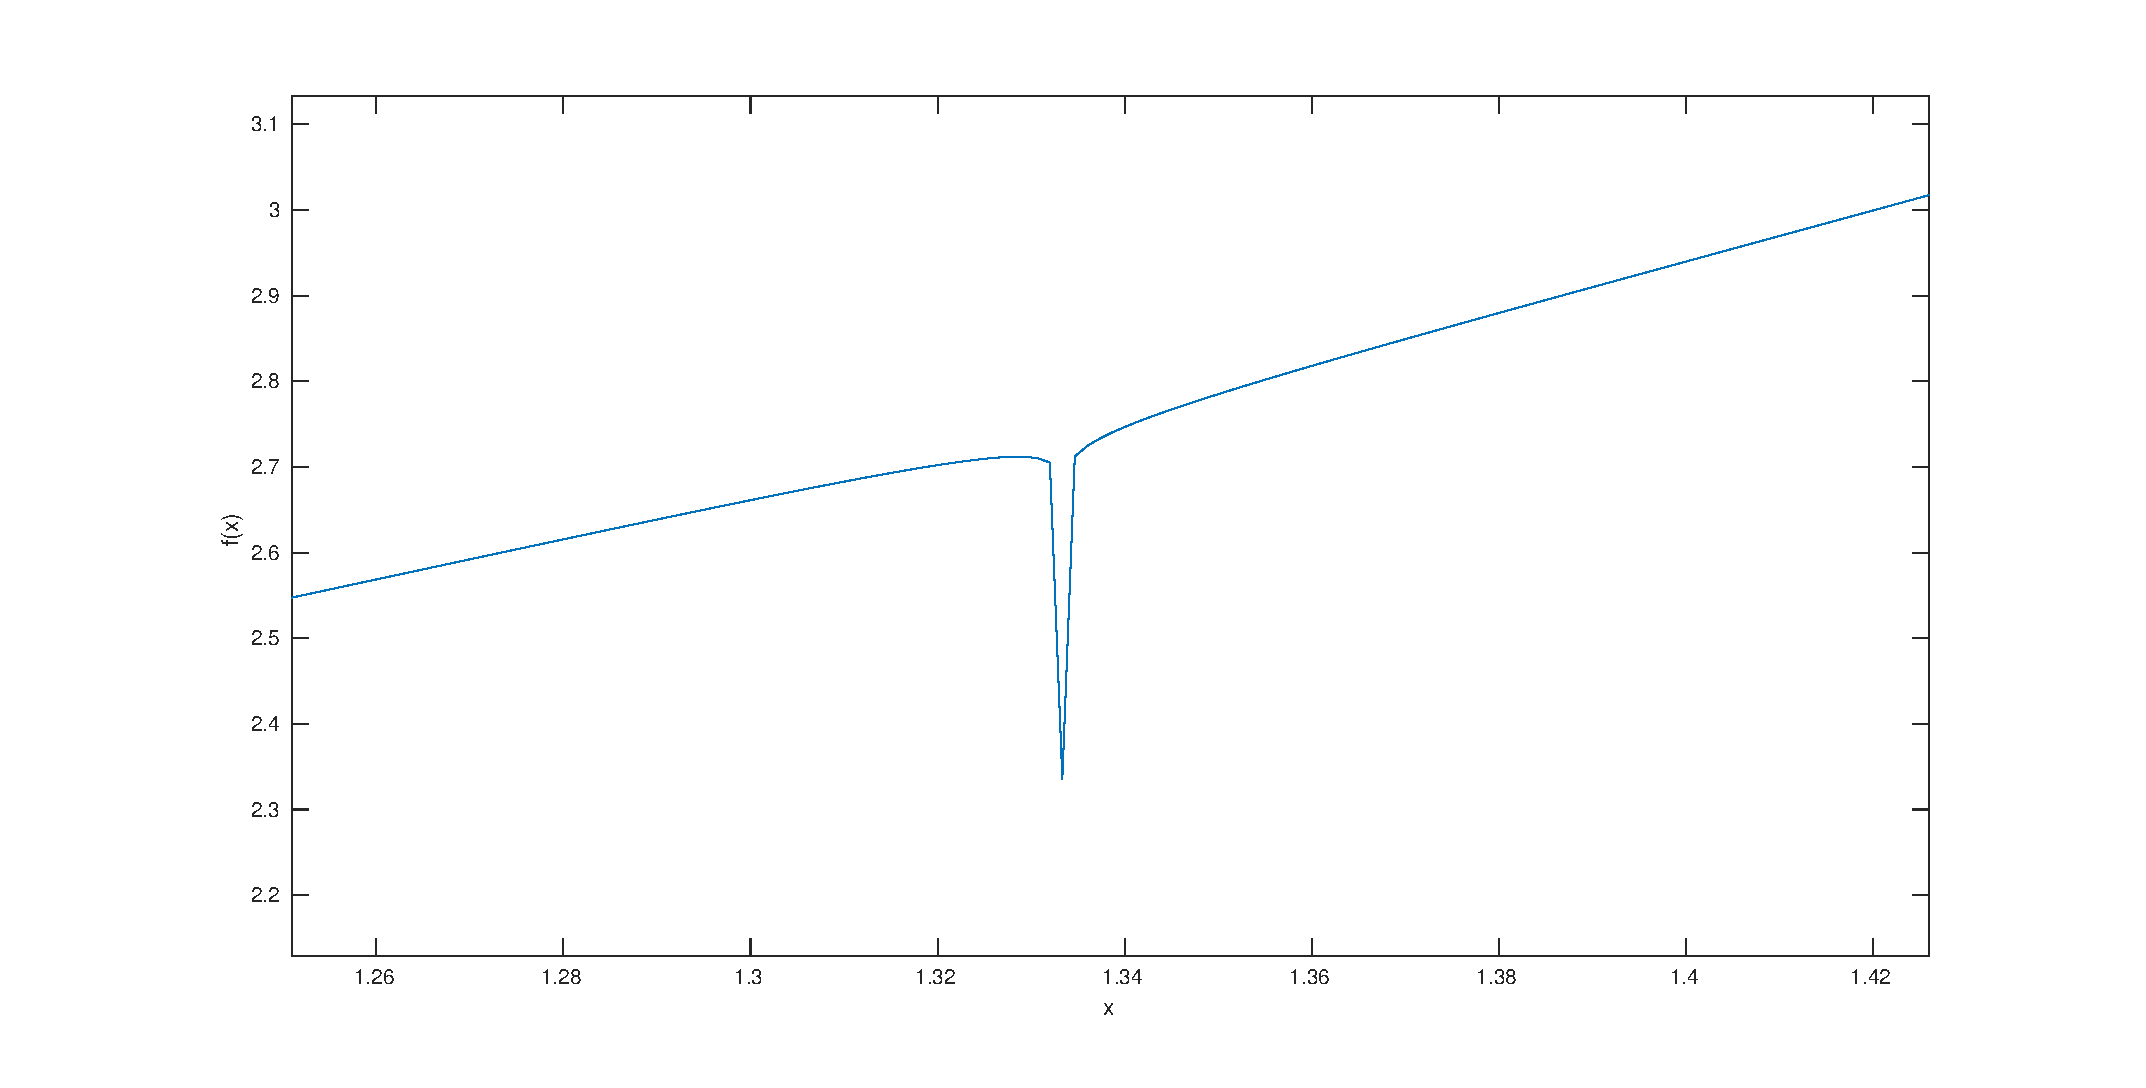
\includegraphics[width=450px]{plot/fes113}
\caption{\texttt{Plot MatLab della funzione $f(x)=\frac{ln(|3(1-x)+1|)}{80}+x^2+1$}}
\end{figure}
Si può notare che l'asintoto verticale in $x=\frac{4}{3}$ non viene rappresentato come tale. Il problema è che stiamo rappresentando dei numeri reali in un calcolatore, quindi la loro rappresentazione comporta delle approssimazioni. In questo caso infatti abbiamo il valore di $4/3$ che è un numero periodico, ma il calcolatore lo dovrà rappresentare con un numero di cifre finite causando un errore di rappresentazione che in questo caso risulta rilevante. Si allega sotto l'output del codice soprastante:
\includegraphics[width=10cm]{cap_1/es13/es113.png}
\end{flushleft}


\newpage
\section{\textbf{Capitolo 2}}
Ecco le function da noi utilizzate nel corso del capitolo :

\begin{itemize}

\item Medoto di bisezione:
\lstinputlisting[language=Matlab]{cap_2/bisezione.m}

\item Metodo di Newton modificato :
\lstinputlisting[language=Matlab]{cap_2/NewtonMod.m}

\item Metodo di accelerazione di Aitken :
\lstinputlisting[language=Matlab]{cap_2/Aitken.m}

\item SecNSqrt.m
\lstinputlisting[language=Matlab]{cap_2/SecNSqrt.m}

\end{itemize}

\subsection{\textbf{Esercizio 2.1}}

\lstinputlisting[language=Matlab]{cap_2/es1/es1.m}
La tabella delle approssimazioni è la seguente:
\begin{center}
\begin{tabular}{c|lc}
i & \( x_i \) \\
\hline
1 & 1.750000000000000e+00 \\
2 & 1.732142857142857e+00 \\
3 & 1.732050810014727e+00 \\
\end{tabular}\\
\end{center}

\subsection{\textbf{Esercizio 2.2}}
La radice da approssimare in questo caso è $\sqrt[n]{2}$ per gli $n=3,4,5$. Il codice MatLab corrispondente è il seguente:
\lstinputlisting[language=Matlab]{cap_2/es2/es2.m}
l'output corrispondente è:
\begin{center}
\begin{tabular}{c|c|c|c}
i & \( n=3 \) & \( n=4 \) & \( n=5\)\\
\hline
1 & 1.631784138709347e+00 & 1.771797299323380e+00 & 1.943788863498140e+00 \\
2 & 1.463411989089094e+00 & 1.463688102853308e+00 & 1.597060655491283e+00 \\
3 & 1.442554125137959e+00 & 1.336940995805593e+00 & 1.369877122538772e+00 \\
4 & 1.442249634601091e+00 & 1.316557487370408e+00 & 1.266284124539191e+00 \\
5 & 1.442249570307411e+00 & 1.316074279204018e+00 & 1.246387399421677e+00 \\
6 & ------------ & 1.316074012952573e+00 & 1.245731630753065e+00 \\
7 & ------------ & ------------ & 1.245730939616284e+00 \\
\end{tabular}
\end{center}
\subsection{\textbf{Esercizio 2.3}}
Per confrontare il metodo delle secanti con quello di Newton abbiamo creato il codice MatLab:
\lstinputlisting[language=Matlab]{cap_2/es3/es3.m}
I risultati ottenuti dall'utilizzo del metodo delle secanti sono: \newline
\\
\scalebox{0.7} {
\begin{tabular}{c|c|c|c|c}
i & metodo di Newton & metodo delle secanti & \big|newton-$\sqrt{2}$\big| & \big|secanti-$\sqrt{2}$\big|\\
\hline
1 & 1.750000000000000e+00 & 1.736842105263158e+00 & 3.357864376269049e-01 & 3.226285428900628e-01 \\
2 & 1.732142857142857e+00 & 1.732142857142857e+00 & 3.179292947697618e-01 & 3.179292947697618e-01 \\
3 & 1.732050810014727e+00 & 1.732050934706042e+00 & 3.178372476416318e-01 & 3.178373723329468e-01 \\
4 & --------- & 1.732050807572255e+00 & ------- & 3.178372451991598e-01\\
\end{tabular}
}
\\ \newline
Si nota dalla tabella che \( \big|newton-\sqrt{2}\big| \approx  \big|secanti-\sqrt{2}\big| \), cioè che l'ordine di grandezza dell'errore assoluto tra i due metodi è lo stesso. Si può quindi affermare che l'uso del metodo di Newton o del metodo delle secanti è equivalente.
\subsection{\textbf{Esercizio 2.4}}
\lstinputlisting[language=Matlab]{cap_2/es4/es4.m}
Questo codice esegue i metodi di Newton, Newton modificato e Aitken per le funzioni date.
Questi sono gli output dei tre metodi numerici:\\
Funzione1:\\
\begin{tabular}{lc}
metodo & output \\
\hline
NewtonMod (m=1) & 3.014159265358980 \\
NewtonMod (m=10)& 3.141592653589793 \\
Aitken & 3.141592653589755 \\
\end{tabular}\\
Funzione2:\\
\begin{tabular}{lc}
metodo & output \\
\hline
NewtonMod (m=1) & 3.014571920744193 \\
NewtonMod (m=10)& 3.145719207441934 \\
Aitken & 3.137995613065127 \\
\end{tabular}\\

\subsection{\textbf{Esercizio 2.5}}
Il metodo di bisezione è applicabile in $f$ se è:
\begin{enumerate}
\item continua nell'intervallo $[a,b]$
\item $f(a)f(b)<0$
\end{enumerate}

\begin{flushleft}
il metodo di bisezione non è possibile utilizzarlo a causa della seconda condizione dato che $f_1(x)=(x-\pi)^{10}>0 \forall x$ e $f_2(x)=e^{2x}(x-\pi)^{10}>0 \forall x$ sono sempre positive quindi non è possibile stabilire un intervallo $[a,b]$ tale che $f(a)f(b)<0$, $\forall a,b \in \mathbb{R}$
\end{flushleft}
 


\subsection{\textbf{Esercizio 2.6}}
\lstinputlisting[language=Matlab]{cap_2/es6/es6.m}
\subsection{\textbf{Esercizio 2.7}}
\lstinputlisting[language=Matlab]{cap_2/es7/es7.m}

I dati generati dall'esecuzione del codice sono esposti  nella seguente tabella

\begin{tabular}{l c r}

n & $tol_x$ & y \\
\hline
0 & $10^{-1}$ & 0.500000000000000 \\
7 & $10^{-2}$ & 0.488281250000000 \\
10 & $10^{-3}$ &  0.488769531250000 \\
13 & $10^{-4}$ & 0.488952636718750 \\
16 & $10^{-5}$ & 0.488945007324219 \\
20 & $10^{-6}$ & 0.488943576812744 \\
21 & $10^{-7}$ & 0.488943815231323 \\
26 & $10^{-8}$ & 0.488943792879581 \\
30 & $10^{-9}$ & 0.488943794276565 \\
32 & $10^{-10}$ & 0.488943794392981 \\
\hline
\end{tabular}


\subsection{\textbf{Esercizio 2.8}}
\begin{flushleft}
Per determinare la radice della funzione data, abbiamo scritto il seguente script MatLab:
\lstinputlisting[language=Matlab]{cap_2/es8/es8.m}
Con risultato in output:
\newline
\includegraphics[width=150px]{cap_2/es8/es28.png}
\newline
Si può vedere che il metodo non converge per il punto iniziale $x0=0$, ma con punto iniziale diverso $x0=4$ il metodo converge. Questo significa che il metodo può convergere localmente. Dobbiamo quindi studiare la convergenza locale della funzione $f(x)$. Tale convergenza risulta essere garantita solo in un intorno della radice, in questo caso in un intorno di $\pi$. Essendo la funzione $f(x) = (x-\pi)\cdot e^{10\cdot x}$ la funzione di iterazione che definisce il metodo è determinata da:
\[
\Phi(x) = x-\frac{(x-\pi)\cdot e^{10\cdot x}}{e^{10\cdot x}\cdot (10\cdot x - 10 \cdot \pi + 1)} = x - \frac{(x-\pi)}{(10\cdot x - 10 \cdot \pi + 1)}
\]
Per convergere localmente si deve avere $\pi$ punto fisso della funzione di iterazione $\Phi(x)$. si ha infatti che:
\[
\Phi(\pi) = \pi - \frac{(\pi-\pi)}{(10\cdot \pi - 10 \cdot \pi + 1)} = \pi - 0 = \pi
\]
Questo conferma il fatto che la funzione $f(x)$ è convergente localmente in un intorno di $\pi$, confermando i risultati ottenuti dallo script precedente.
\end{flushleft}


\newpage
\section{\textbf{Capitolo 3}}
\subsection{\textbf{Esercizio 3.1}}
Una matrice \( L \in M_{n \times n} \) si dice triangolare inferiore se \( l_{i,j}=0, \forall i<j \) con \(i,j = 1...n \) ed \( l_{i,j} \in L \).
\\
Date due matrici triangolari inferiori \( L,K \in M_{n \times n} \) la loro somma sar\'a di nuovo una matrice traingolare inferiore \( N \in M_{n \times n} \):
\[
 \forall i<j, \hspace{5pt} l_{i,j} + k_{i,j} = 0 + 0 = 0. 
\]
\\
Una matrice \( U \in M_{n \times n} \) si dice triangolare superiore se \( u_{i,j}=0, \forall i>j \) con \(i,j = 1...n \) ed \( u_{i,j} \in U \).
Date due matrici triangolari superiori  \( U,W \in M_{n \times n} \)  il loro prodotto  \( Z \in M_{n \times n} \):
\[
z_{i,j} = \sum_{k=1}^n u_{i,k} w_{k,j}, \hspace{35pt} \forall i,j \in [1,..,n].
\]
sar\'a di nuovo una matrice triangolare superiore, dal momento che 
\[
z_{i,j} =  \sum_{k=1}^n u_{i,k} w_{k,j} =  \underbrace{ \sum_{k=1}^{i-1} u_{i,k} w_{k,j} }_\text{=0 per k<i}  + \sum_{k=i}^n u_{i,k} w_{k,j} = \sum_{k=i}^n u_{i,k} w_{k,j}.
\]
Dal momento che in quest'ultimo termine abbiamo \( k \geq i \) se \( i>j \) allora \( k>j \), da cui la definizione di matrice triangolare superiore.

\subsection{\textbf{Esercizio 3.2}}
\begin{flushleft}
Una matrice triangolare inferiore $L \in M_{n \times n}$ è detta a diagonale unitaria se i suoi elementi sulla diagonale sono pari a 1:
\[
l_{i,i}=1 \hspace{15pt} \forall i \in [1,..,n] 
\]
Prendiamo una seconda matrice $K \in M_{n \times n}$ triangolare inferiore a diagonale unitaria, calcoliamo il prodotto tra $K$ e $L$:
\[
\sum_{m=1}^n l_{i,m} \cdot k_{m,j} = \underbrace{ \sum_{i<j} l_{i,m} \cdot k_{m,j} }_{0} + \underbrace{ \sum_{i=j} l_{i,m} \cdot k_{m,i} }_{1} + \sum_{i>j} l_{i,m}\cdot k_{m,j}
\]
La risultante matrice assume valori:
\begin{itemize}
\item $\sum_{i<j} l_{i,m} \cdot k_{m,j} = 0 \hspace{15pt} \forall i,j \in [1,..,n] $ 
\item $\sum_{i=j} l_{i,m} \cdot k_{m,j} = 1 \hspace{15pt} \forall i,j \in [1,..,n] $ 
\item $\sum_{i>j} l_{i,m} \cdot k_{m,j} \in  \mathbb{R} \hspace{15pt} \forall i,j \in [1,..,n] $ 
\end{itemize}
che non è altro che la definizione di matrice triangolare inferiore a diagonale unitaria, come volevamo dimostrare.\\

(Allo stesso modo si può dimostrare per matrici triangolari superiori).
\end{flushleft}
\subsection{\textbf{Esercizio 3.3}}
Sia $A \in M_{n \times n}$ una matrice triangolare superiore non singolare.\\
Se $A$ \'e invertibile allora pu\'o essere scritta come $A=D(\mathit{I_n}+U)$ dove $D$ \'e una matrice diagonale per cui vale $diag(D)=diag(A)$, $\mathit{I_n}$ \'e la matrice identit\'a ed $U$ \'e una matrice triangolare strettamente superiore ($diag(U)=0$).\\
Per le propriet\'a delle matrici triangolari strettamente superiori si ha che $U^n = 0$ (ovvero che la matrice $U$ \'e nilpotente), mentre per le propriet\'a delle matrici diagonali si ha che $D^{-1}$ \'e ancora una matrice diagonale.
\\
Volendo provare che $A^{-1}=(\mathit{I_n}+U)^{-1}D^{-1}$ espandiamo in serie $ (\mathit{I_n}+U)^{-1}$:
\[
(\mathit{I_n}+U)^{-1}=\mathit{I_n}-U+U^2-...+(-1)^{n-1}U^{n-1}.
\]
Essendo questa una serie di somme e prodotti di matrici triangolari superiori la matrice inversa $A^{-1}$ sar\'a in generale una matrice triangolare superiore.


\subsection{\textbf{Esercizio 3.4}}
\begin{flushleft}
L'eliminazione nella prima colonna richiede $n$ somme ed $n$ prodotti per $n-1$ righe, quindi in totale $(n+n)(n-1) = 2n(n-1)$ \texttt{flops}. L'eliminazione della seconda richiede $n-1$ somme ed $n-1$ prodotti per $n-2$ righe, quindi in totale $[(n-1)+(n-1)](n-2) = 2(n-1)(n-2)$ \texttt{flops}.\\
Procedendo per induzione si ha che il numero totale di operazioni \'e
\[
\sum_{i=0}^{n} 2(n-i)(n-i+1).
\]
Operando la sostituzione $j = n-i+1$ si ha che la somma diviene :
\[
2 \sum_{j=n+1}^{1} j(j-1) = 2\Big( \sum_{j=1}^{n+1}j^2 + \sum_{j=1}^{n+1}j\Big) = 2\Big(\sum_{j=1}^{n-1}j^2 + n^2 + (n+1)^2 + \sum_{j=1}^{n-1}j +n +n+1 \Big) =
\]
\[
= 2\Big( \frac{n\cdot (n-1)\cdot(2n-2)}{6} + \frac{n\cdot(n-1)}{2} + 2n^2 +3n +2 \Big) = 2\Big(\frac{2n^3-4n^2+2n}{6} +\frac{n^2-n}{2} + 2n^2 +3n +2\Big) \leq \frac{2}{3}\cdot n^3
\]
\\

quindi si ha che il numero di flop è $\frac{2}{3}\cdot n^3$, come volevamo dimostrare
\end{flushleft}
\subsection{\textbf{Esercizio 3.5}}
\lstinputlisting[language=Matlab]{cap_3/LUP.m}

\subsection{\textbf{Esercizio 3.6}}
\lstinputlisting[language=Matlab]{cap_3/solveLinearLUP.m}

\subsection{\textbf{Esercizio 3.7}}
\begin{flushleft}
Per essere SDP una matrice $A \in \mathbb{R}^{n \times n}$ deve sottostare a due proprietà:
\begin{itemize}
    \item
    deve essere simmetrica, cioè $A=A^T$;
    \item 
    $\forall x \in \mathbb{R}^n$ tale che $x \neq 0$ vale $x^TAx>0$
\end{itemize}
La matrice $A$ essendo non singolare è anche SDP.
Le matrici $AA^T$ e $A^TA$ per essere SDP devono dimostrare le proprietà sopra:
\begin{itemize}
    \item simmetriche: 
    \[
    (AA^T)^T = (A^T)^TA^T = AA^T
    \]
    \[
    (A^TA)^T = A^T(A^T)^T = A^TA.
    \]
    \item definite positive:
    \[
    x^TAA^Tx = xx^TAA^Txx^T = x(A^Tx)^T(x^TA)^Tx^T = (\underbrace{x^TA^Tx}_{>0})^T \cdot (\underbrace{x^TAx}_{>0})^T > 0
    \]
    \[
    x^TA^TAx = xx^TA^TAxx^T = x(Ax)^T(x^TA^T)^Tx^T = (\underbrace{x^TAx}_{>0})^T \cdot (\underbrace{x^TA^Tx}_{>0})^T > 0
    \]
\end{itemize}
possiamo quindi affemrare che le matrici $AA^T$ e $A^TA$ sono SDP.
\end{flushleft}
\subsection{\textbf{Esercizio 3.8}}
Se $A \in M_{m \times n}$ con $m \geq n = rank(A)$ allora diremo che $A$ ha rango massimo.
\\
Questo comporta che la matrice sia invertibile, ovvero che il suo determinante $\det(A) \neq 0$. La matrice \'e quindi nonsingolare e di conseguenza simmetrica definita positiva, dalla dimostrazione dell'esercizio \textbf{3.7}.

\subsection{\textbf{Esercizio 3.9}}
Si ha ovviamente che
\[
A = \frac{1}{2}(A+A^T) + \frac{1}{2}(A-A^T)=\frac{1}{2}A + \frac{1}{2}A^T + \frac{1}{2}A - \frac{1}{2}A^T
\]
\\
Definendo $A_s \doteq \frac{1}{2}(A+A^T)$ si mostra come $A_s = A_s^T$ infatti
\[
\frac{1}{2}(A+A^T) = [ \frac{1}{2}(A+A^T)]^T = \frac{1}{2}(A+A^T)^T = \frac{1}{2}(A^T+(A^T)^T) = \frac{1}{2}(A+A^T)^T.
\]
\\
Da cui $A_s$ \'e detta parte \textbf{simmetrica} di $A$.
\\
Definendo $A_a \doteq \frac{1}{2}(A-A^T)$ si mostra come $A_a = -A_a^T$ infatti
\[
\frac{1}{2}(A-A^T) = -\frac{1}{2}(A-A^T)^T = -\frac{1}{2}(A^T-(A^T)^T) = -\frac{1}{2}(A^T-A) = \frac{1}{2}(A-A^T).
\]
Da cui $A_a$ \'e detta parte \textbf{antisimmetrica} di $A$.
\\
Dato poi un generico vettore $\mathbf{x} \in \mathbf{R}^n$ si ha che $\mathbf{x}^TA\mathbf{x} = \mathbf{x}^TA_s\mathbf{x}$ infatti
\[
\mathbf{x}^TA\mathbf{x} = \mathbf{x}^T(A_s + A_a)\mathbf{x} = \mathbf{x}^TA_s\mathbf{x} + \mathbf{x}^TA_a\mathbf{x} = \frac{1}{2}(\mathbf{x}^TA\mathbf{x} + \mathbf{x}^TA^T\mathbf{x}) + \frac{1}{2}(\mathbf{x}^TA\mathbf{x} - \mathbf{x}^TA^T\mathbf{x}).
\]
Analizzando l'ultimo termine $\frac{1}{2}(\mathbf{x}^TA\mathbf{x} - \mathbf{x}^TA^T\mathbf{x})$ si nota come
\[ \frac{1}{2}(\mathbf{x}^TA\mathbf{x} - \mathbf{x}^TA^T\mathbf{x}) = \frac{1}{2}(\mathbf{x}^TA\mathbf{x} - (A\mathbf{x})^T\mathbf{x})=0
\]
\\
dal momento che, definendo $A\mathbf{x}=\mathbf{y}$ si ha $\mathbf{x}^T\mathbf{y}= \mathbf{y}^T\mathbf{x}.$
Da cui la tesi.  $\qedsymbol$

\subsection{\textbf{Esercizio 3.10}}
\begin{flushleft}
Prendiamo $i \in [1,...,n]$ colonne della matrice, possiamo vedere che l'algoritmo esegue $i-1$ somme di 2 prodotti quindi $2(i-1)$ e in più esegue un'operazione di sottrazione e una di divisione che equivale a 2 flop. Queste operazioni vengono eseguite per $n-i$ volte, cioè per ogni colonna della matrice, il che significa che il numero di flop sono:
\[
\sum_{i=1}^{n}2(n-i)(i-1) = 2\cdot\sum_{i=1}^{n}(i\cdot n-n-i^2+i) = 2\cdot \Big[(n+1)\sum_{i=1}^{n}i-n^2-\sum_{i=1}^{n}i^2\Big] = 
\]
\[
= 2\cdot \Big[(n+1)\cdot n + \frac{(n+1)(n-1)n}{2} - n^2 - n^2 - \frac{n(n-1)(2n-1)}{6}\Big] = 2\cdot \Big(n - n^2 + \frac{n^3-n}{2} -\frac{2n^3-3n^2+n}{6} \Big) =
\]
\[
= 2\cdot \Big[n^3 \cdot \Big(\frac{1}{2} - \frac{1}{3}\Big) + n^2 \cdot \Big(-1 + \frac{1}{6} + \frac{1}{2}\Big) + n \cdot \Big(1-\frac{1}{2}-\frac{1}{6}\Big) \Big]= \frac{2}{6} n^3 + \frac{2}{3} n^2 + \frac{2}{3} n \approx \frac{1}{3}n^3
\]
quindi l'algoritmo di fattorizzazione $LDL^T$ ha un costo di $\frac{n^3}{3} flop$.
\end{flushleft}
\subsection{\textbf{Esercizio 3.11}}
\begin{flushleft}
L'algoritmo di fattorizzazione $LDL^T$ da noi implementato è il seguente:
\lstinputlisting[language=matlab]{cap_3/factLDLT.m}
è possibile vedere il funzionamento di questa function nell'esercizio \pageref{es313}.
\end{flushleft}
\subsection{\textbf{Esercizio 3.12}}
Il codice MatLab corrispondente alla risoluzione di un sistema lineare con matrice di ingresso fattorizzata LDLT è il seguente:
\lstinputlisting[language=matlab]{cap_3/linLDLT.m}
\subsection{\textbf{Esercizio 3.13}}
\label{es313}
\begin{flushleft}
Per verificarlo abbiamo usato il seguente codice MatLab:
\lstinputlisting[language=Matlab]{cap_3/es13/es13.m}
Che restituisce l'output:
\includegraphics[width=\textwidth]{cap_3/es13/es313.png}
L'output è molto chiaro, la seconda matrice $A_{2}$ non può essere fattorizzata $LDL^T$ di conseguenza non è $SDP$.
\end{flushleft}


\subsection{\textbf{Esercizio 3.14}}
\label{es314}
\begin{flushleft}
In entrambi i casi abbiamo usato la matrice $A\in M^{3\times 3}$ con elementi:
\[ 
A =
\begin{pmatrix}
    15  & -3 &  2 \\
   -4  &  9  &  2 \\
    6  &  0  &  10 \\
\end{pmatrix}
\]
e il vettore dei termini noti $b\in \mathbb{R}^3$ con valori:
\[
{b} = (3.2, 2.3, 3.1)^T
\]
Usando il codice MatLab sottostante è possibile risolvere questi 2 esempi:
\newpage
\lstinputlisting[language=Matlab]{cap_3/es14/es14.m}
Il codice sopra restituisce l'output:
\begin{figure}[h]
\includegraphics[left, width=400px]{cap_3/es14/es314.png}
\end{figure}
La soluzione ottenuta 
\end{flushleft}
\subsection{\textbf{Esercizio 3.15}}
\lstinputlisting[language=Matlab]{cap_3/es15/es15.m}

\subsection{\textbf{Esercizio 3.16}}
\begin{flushleft}
Abbiamo implementato il codice seguente per poter rispondere alle domande dell'esercizio:
\lstinputlisting[language=Matlab]{cap_3/es16/es16.m}
Possiamo confermare che le soluzioni $x$ e $y$ dei sistemi lineari $A\cdot x = b$ e $A\cdot y = c$ sono giuste dato che calcolando i loro residui otteniamo:
\begin{figure}[h]
\includegraphics[left, width=250px]{cap_3/es16/es316}
\end{figure}
\newline \\
Nel passo successivo si usa la serie di istruzioni forniteci dall'esercizio. Nel caso del vettore $x$ si perviene alla stessa soluzione precedentemente fornita dall'esercizio. Invece nel caso del vettore $y$ abbiamo una propagazione degli errori nella soluzione trovata, che si può vedere a partire dall'elemento $y_7$. Possiamo vederlo dall'output:
\begin{figure}[h]
\includegraphics[left, width=250px]{cap_3/es16/es316a}
\end{figure}
\newline \\
Si vede che c'è una perturbazione sulla soluzione che è possibile spiegare andando a studiare la seguente disuguaglianza:
\[
\frac{\left|\left|\Delta x\right|\right|}{\left|\left|x\right|\right|} \leq k(A) \cdot \left(\frac{\left|\left|\Delta c\right|\right|}{\left|\left|c\right|\right|} + \frac{\left|\left|\Delta A\right|\right|}{\left|\left|A\right|\right|}\right) = k(A) \cdot \left(\frac{\left|\left|\Delta c\right|\right|}{\left|\left|0.1\cdot b\right|\right|} + \frac{\left|\left|\Delta A\right|\right|}{\left|\left|A\right|\right|}\right) = 
\]
\[
= k(A) \cdot \left(\frac{\left|\left|\Delta c\right|\right|}{10^{-1}\cdot\left|\left|b\right|\right|} + \frac{\left|\left|\Delta A\right|\right|}{\left|\left|A\right|\right|}\right) = k(A) \cdot \left(10\cdot\frac{\left|\left|\Delta c\right|\right|}{\left|\left|b\right|\right|} + \frac{\left|\left|\Delta A\right|\right|}{\left|\left|A\right|\right|}\right) 
\]
Considerato che:
\begin{itemize}
    \item $\frac{\left|\left|\Delta x\right|\right|}{\left|\left|x\right|\right|}$ può essere assimilato ad una sorta di errore relativo sul risultato
    \item $\frac{\left|\left|\Delta A\right|\right|}{\left|\left|A\right|\right|}$ e $\frac{\left|\left|\Delta c\right|\right|}{\left|\left|c\right|\right|}$ possono essere assimilati ai corrispondenti errori relativi sui dati in ingresso
\end{itemize}
dato che il numero di condizionamento del problema è $k(A)=1.0202\cdot10^{20}$, che è $>>1$ (calcolato nell'esercizio precedente a pag. \pageref{es315}), allora la matrice è mal condizionata.
\end{flushleft}
\subsection{\textbf{Esercizio 3.17}}
\lstinputlisting[language=matlab]{cap_3/factQRH.m}
\subsection{\textbf{Esercizio 3.18}}
\lstinputlisting[language=Matlab]{cap_3/solveQR.m}

\subsection{\textbf{Esercizio 3.19}}
\lstinputlisting[language=Matlab]{cap_3/es19/es19.m}

\subsection{\textbf{Esercizio 3.20}}
Risolviamo il sistema di equazioni non lineari applicando il metodo di Newton.
La funzione data è \[F(x_1, x_2)= \begin{cases}x_2-cos(x_1)\\ x_1x_2 -1/2\end{cases}\]
Vogliamo trovare $F(x_1, x_2)=0$ partendo da $x_1(0) = 1\mbox{, } x_2(0) = 1$\\
Troviamo quindi il Jacobiano della funzione: \( J=\begin{pmatrix} sin(x_1) & 1  \\\ x_1 & x_2 \end{pmatrix} \)\\
Applicando il metodo di Newton si va a risolvere:
$\begin{cases} J_F(\underline{x}^{(k)})\underline{d}^{(k)}=-F(\underline{x}^{(k)}) \\ \quad \underline{x}^{(k+1)}=\underline{x}^{(k)}+\underline{d}^{(k)} \end{cases}$\\
Troviamo quindi: $x_1 = 0.6100 \mbox{ e } x_2 =0.8196$

Il codice matlab per il calcolo del minimo è:
\lstinputlisting[language=Matlab]{cap_3/es20/es20.m}

Il codice matlab per la risoluzione di sistemi di equazioni non lineari mediante Newton è:
\lstinputlisting[language=Matlab]{cap_3/NewtonNL.m}

\begin{tabular}{l|c|r}
i & $x_1,x_2$ & norma dell'incremento \\
\hline
1 & 0.7458, 0.7542 & 0.5001 \\
2 & 0.5531, 0.8653 & 0.3145 \\
3 & 0.6042, 0.8241 & 0.0929 \\
4 & 0.6100, 0.8197 & 0.0102 \\
5 & 0.6100, 0.8196 & 0.00013 \\ 


\end{tabular}

\subsection{\textbf{Esercizio 3.21}}
Un punto stazionario $(\hat{x_1}, \hat{x_2})$ è tale per cui $J(\hat{x_1},\hat{x_2})=0$. Si ottiene quindi il sistema non lineare:
$$F(\underline{x})=\underline{0}\mbox{ con }F=\begin{pmatrix}\frac{\partial f}{\partial x_1}\\\frac{\partial f}{\partial x_2}\end{pmatrix}=\begin{pmatrix}4x_1^3+2x_1+x_2\\x_1+2x_2-2\end{pmatrix}.$$
Troviamo il Jacobiano della funzione: \( J=\begin{pmatrix} 12x_1^2+2 & 1  \\\ 1 & 2 \end{pmatrix} \)\\

Troviamo quindi $$\min{f(x_1,x_2)}\approx -0.2573\mbox{ in }(0.4433, -1.2217).$$

Il codice matlab per il calcolo del minimo è:
\lstinputlisting[language=Matlab]{cap_3/es21/es21.m}





\end{document}
